\section{Einleitung}
Der vorliegende Projektbericht behandelt monokulare Tiefenkriterien und ihre Verwendung zur Gestaltung einer Webseite, die einen dreidimensionalen Eindruck hervorruft. Die Ausarbeitung beschäftigt sich mit den Fragestellungen, was monokulare Tiefenkriterien sind, welche monokularen Tiefenkriterien existieren und wie sie zur Gestaltung einer Webseite genutzt werden können, um einen dreidimensionalen Eindruck hervorzurufen.\marginnote{SG}

Nach Erarbeitung der Stichwortliste für die Recherche, werden monokularen Tiefenkriterien erläutert und mit Beispielen dargestellt. Zu den Kriterien wird ein möglicher Anwendungsbereich für Elemente einer Webseite gezeigt. Auf Basis der Kriterien wird ein Konzept für eine Webseite entwickelt und eine beispielhafte Umsetzung gezeigt. Abschließend werden die Ergebnisse kurz zusammengefasst und reflektiert.\marginnote{SG}

\section{Erarbeitung der Stichwortliste}
Reduziert man die Problemstellung auf ihre Substantive und Adjektive, erhält man eine erste Auflistung von Suchbegriffen zur Kombination von Suchanfragen: 'Webseite', '3D-Eindruck', 'Verwendung', 'monokularer', 'Tiefenkriterien'. Reduziert man die Worte auf ihren Wortstamm, bezieht Synonyme oder ähnliche Begriffe mit ein, bildet durch verschiedene Kombinationen Wortgruppen und bezieht auch die englische Übersetzungen mit ein, erhält man folgende Stichwortliste.\marginnote{SG}
\begin{itemize}
\item monokular
\item monoskopisch
\item Tiefenkriterium
\item 3D Webseite
\item Verwendung monokularer Tiefenkriterien
\item 3D-Eindruck
\item 3D-Wahrnehmung
\item dreidimensionales Sehen
\item Stereoskopisches Sehen
\item monokulares Sehen
\item monokulare Hinweisreize
\item monokulares Tiefensehen
\item monokulare Schätzmechanismen
\item monokulare Raumwahrnehmung
\item monoskopisches Tiefensehen
\item monoskopische Schätzmechanismen
\item monoskopische Raumwahrnehmung
\item Monovision
\item monocular depth cues
\item monocular vision
\item 3D website
\item monocular depth perception
\item depth perception
\item depth vision
\item stereoscopic vision
\item 3-dimensional vision
\item 3-dimensional perception
\end{itemize}

\section{Monokulare Tiefenkriterien}
\marginnote{DD}
\todo{Ursprung in die spezifischen Kapitel aufteilen? - Sofern sinnvoll - z.Zt. fraglich}
Je nach Quelle lassen sich verschiedene monokulare Tiefenkriterien ermitteln. Im wesentlichen handelt es sich bei diesen Unterschieden aber eher um Detailierungsgrade. Je detailierter diese Kriterien unterschieden werden, desto mehr existieren und umgekehrt. Lt. \cite{heidXX} existieren die folgenden monokularen Tiefenkriterien:

\begin{itemize}
\item Verdeckung und Überlappung,
\item Schatten,
\item Vertraute Größe,
\item Relative Helligkeit und perspektivische Unschärfe,
\item Texturdichte-Gradient sowie
\item Relative Höhe / Lage zum Horizont
\end{itemize}

Den oben aufgeführten Kriterien fügt \cite{leyh10} zudem noch die lineare Perspektive hinzu. Weiterhin erwähnt \cite{Gras16} die Bewegungsparallaxe.

\subsection{Verdeckung und Überlappung}
\marginnote{DD}
Das Kriterium Verdeckung und Überlappung lässt den Betrachter Tiefenunterschiede wahrnehmen. Dadurch, dass ein Objekt ein anderes überdeckt kann davon ausgegangen werden, dass wenigstens eine weitere Tiefenebene existiert und dass das verdeckende Objekte näher zum Betrachter ist, als das verdeckte Objekt.\footcite[Vgl.]{heidXX}

\vspace{1em}
\begin{minipage}{\linewidth}
	\centering
	
\includegraphics[width=0.7\linewidth]{images/verdeckung.jpg}
	\captionof{figure}[verdeckung]{Verdeckung}
	\label{fig:verdeckung}
\end{minipage}
\vspace{1em} 

In Abbildung \ref{fig:verdeckung} wird das Kriterium der Verdeckung und Überlappung anhand von zwei Rechtecken dargestellt. Das schwarze Rechteck überlagert das rote Rechteck, wodurch der Eindruck vermittelt wird, dass Ersteres auf der Tiefenebene vor dem Letzterem liegt. Das schwarze Rechteck liegt also näher am Betrachter.\\

Dieses Kriterium findet sich in vielen modernen Anwendung und Websites wieder. Der offensichtlichste Anwendungsfall sind sog. Dialog-Fenster.

\vspace{1em}
\begin{minipage}{\linewidth}
	\centering
	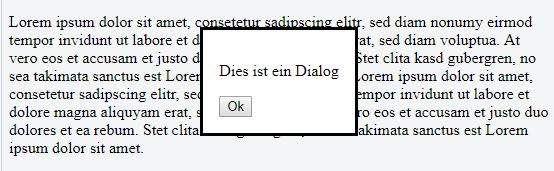
\includegraphics[width=0.7\linewidth]{images/dialog_fenster.jpg}
	\captionof{figure}[dialog-fenster]{Bsp. eines einfachen Dialog-Fensters}
	\label{fig:dialog-fenster}
\end{minipage}
\vspace{1em} 

Abb. \ref{fig:dialog-fenster} zeigt ein solches Beispiel. Hier wird ein neues Fenster über existierende Inhalte gelegt. Dadurch entsteht der Eindruck, dass das Dialog-Fenster vor dem eigentlichen Inhalt liegt.

\begin{figure}[!ht]
\centering
\fbox{
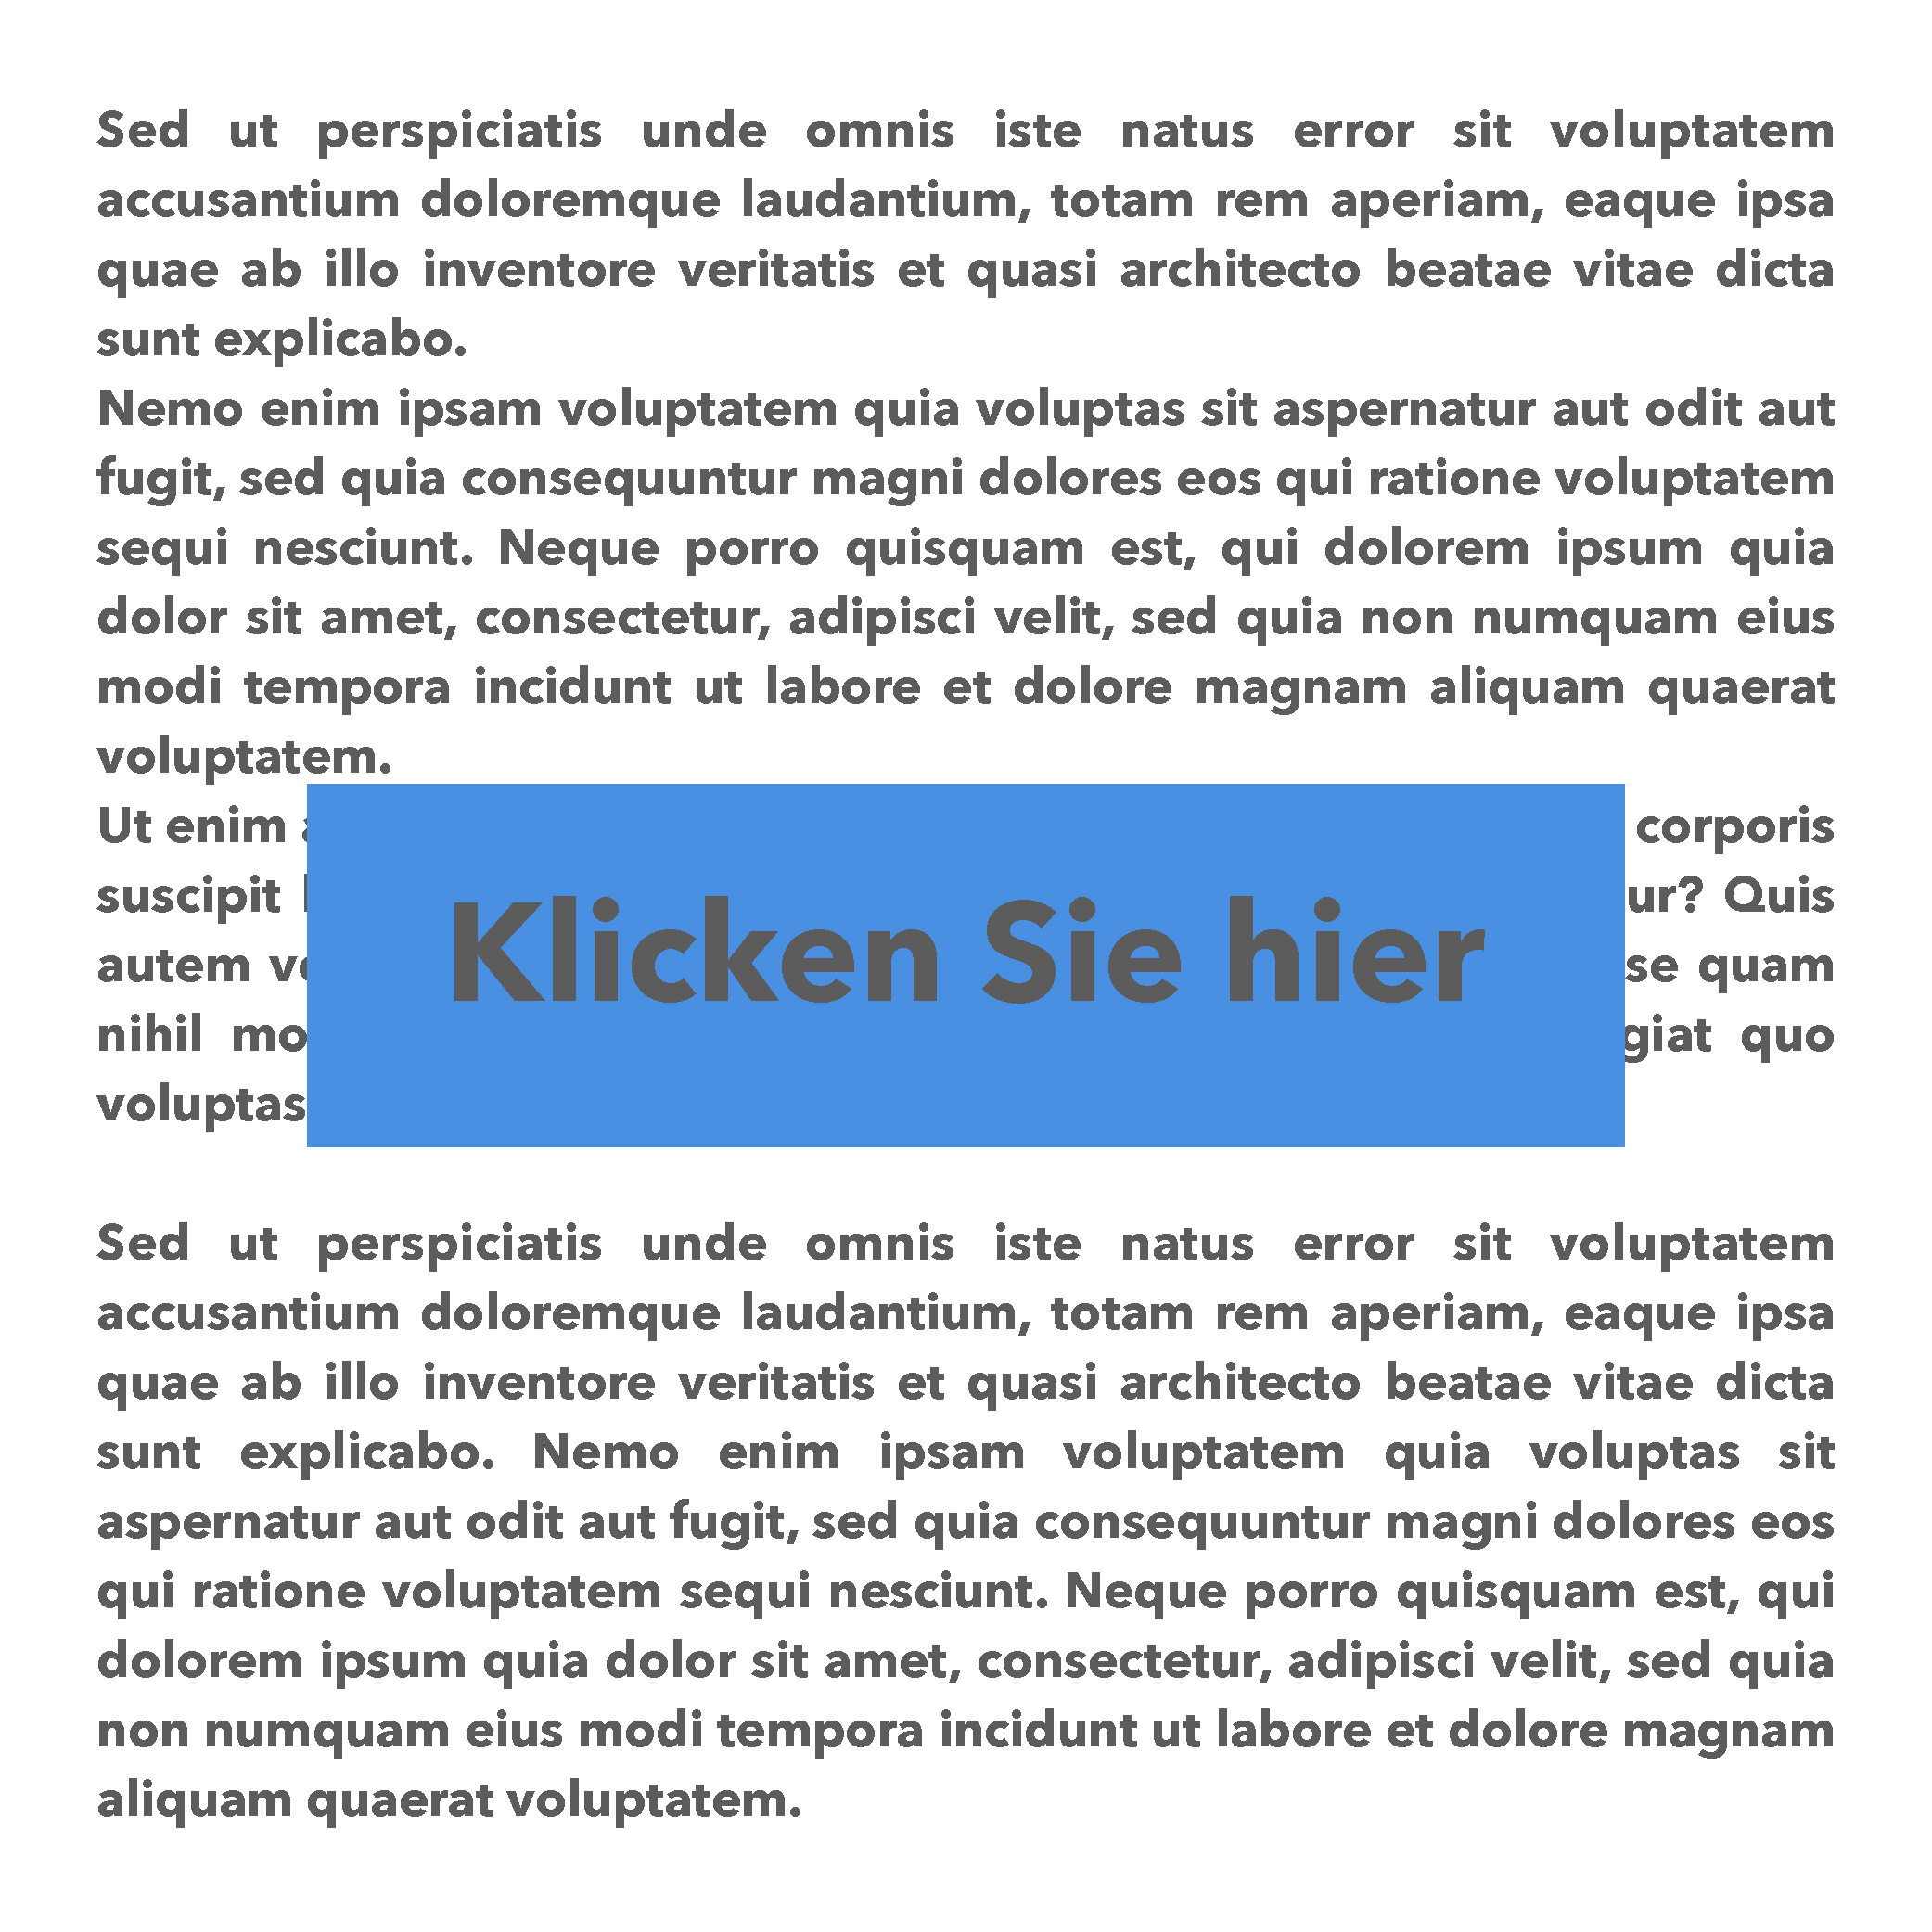
\includegraphics[width=0.60\textwidth]{images/sample_verdeckung.pdf}
}
\caption[Verdeckung von Text durch einen Button]{Verdeckung von Text durch einen Button\\ Eigene Darstellung}
\label{sample_verdeckung}
\end{figure}

\subsection{Schatten}
\marginnote{DD}
Das Schatten-Kriterium beschreibt, dass ein Betrachter anhand der Länge der Schatten zweier Objekte auf die relative Größe beider Objekte zueinander schließen kann. Ist der Schatten von Objekt A länger als der von Objekt B, ist B größer als A.\footcite[Vgl.][S.43]{Gras16} Voraussetzung dafür ist allerdings, dass beide Schatten unter den selben Bedingungen entstehen.\\

\vspace{1em}
\begin{minipage}{\linewidth}
	\centering
	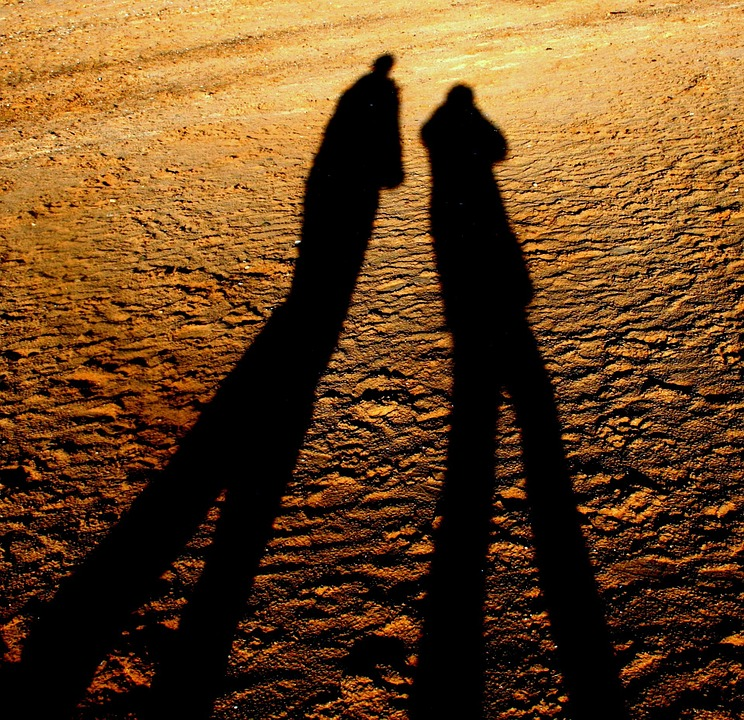
\includegraphics[width=0.7\linewidth]{images/schatten_personen.jpg}
	\captionof{figure}[schatten-relativ]{Schatten zweier Personen (\cite{PixaXX})}
	\label{fig:schatten-relativ}
\end{minipage}
\vspace{1em} 

Abbildung \ref{fig:schatten-relativ} zeigt diesen Sachverhalt. Anhand der Schatten der beiden Personen, lässt sich darauf schließen, dass die rechte Person vermutlich kleiner ist als die linke Person.\\
\\
Außerdem lassen sich durch die Ausrichtung der Schatten  'räumliche Beschaffenheiten' erschließen, wie Abbildung \ref{fig:schatten-raum} zeigt.\footcite[Vgl.]{heidXX} Abbhängig davon, wie die Schatten fallen, ändert sich die Perspektive auf das Objekt.

\vspace{1em}
\begin{minipage}{\linewidth}
	\centering
	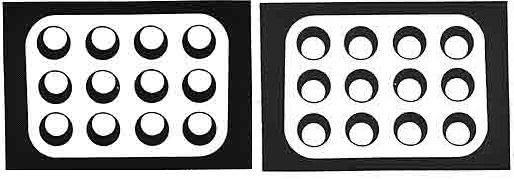
\includegraphics[width=0.7\linewidth]{images/schatten01.jpg}
	\captionof{figure}[schatten-raum]{Räumliche Beschaffenheit (\cite{heidXX})}
	\label{fig:schatten-raum}
\end{minipage}
\vspace{1em}

Wie auch das Kriterium Verdeckung und Überlappung, finden sich Schatten in vielen modernen Anwendungen. Abb. \ref{fig:karten-schatten} zeigt ein solches Bsp.

\vspace{1em}
\begin{minipage}{\linewidth}
	\centering
	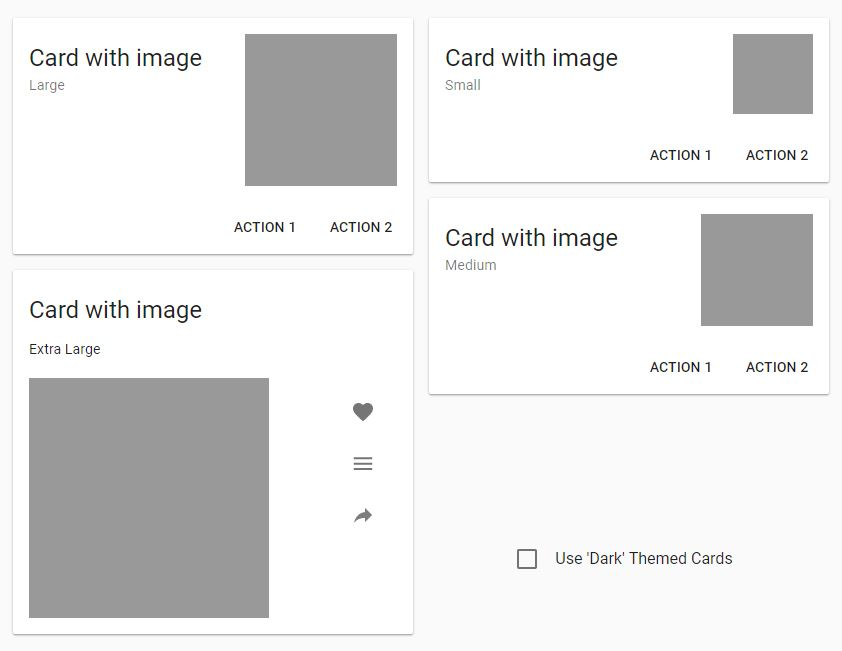
\includegraphics[width=0.7\linewidth]{images/karten_schatten.jpg}
	\captionof{figure}[karten-schatten]{Schatten im Kartenlayout (\cite{goo17})}
	\label{fig:karten-schatten}
\end{minipage}
\vspace{1em}

Hier werden die Schatten genutzt um die Elemente vom Hintergrund hervorzuheben und sie so jeweils besser als eigenständiges Objekt sichtbar zu machen.

\begin{figure}[!ht]
\centering
\fbox{
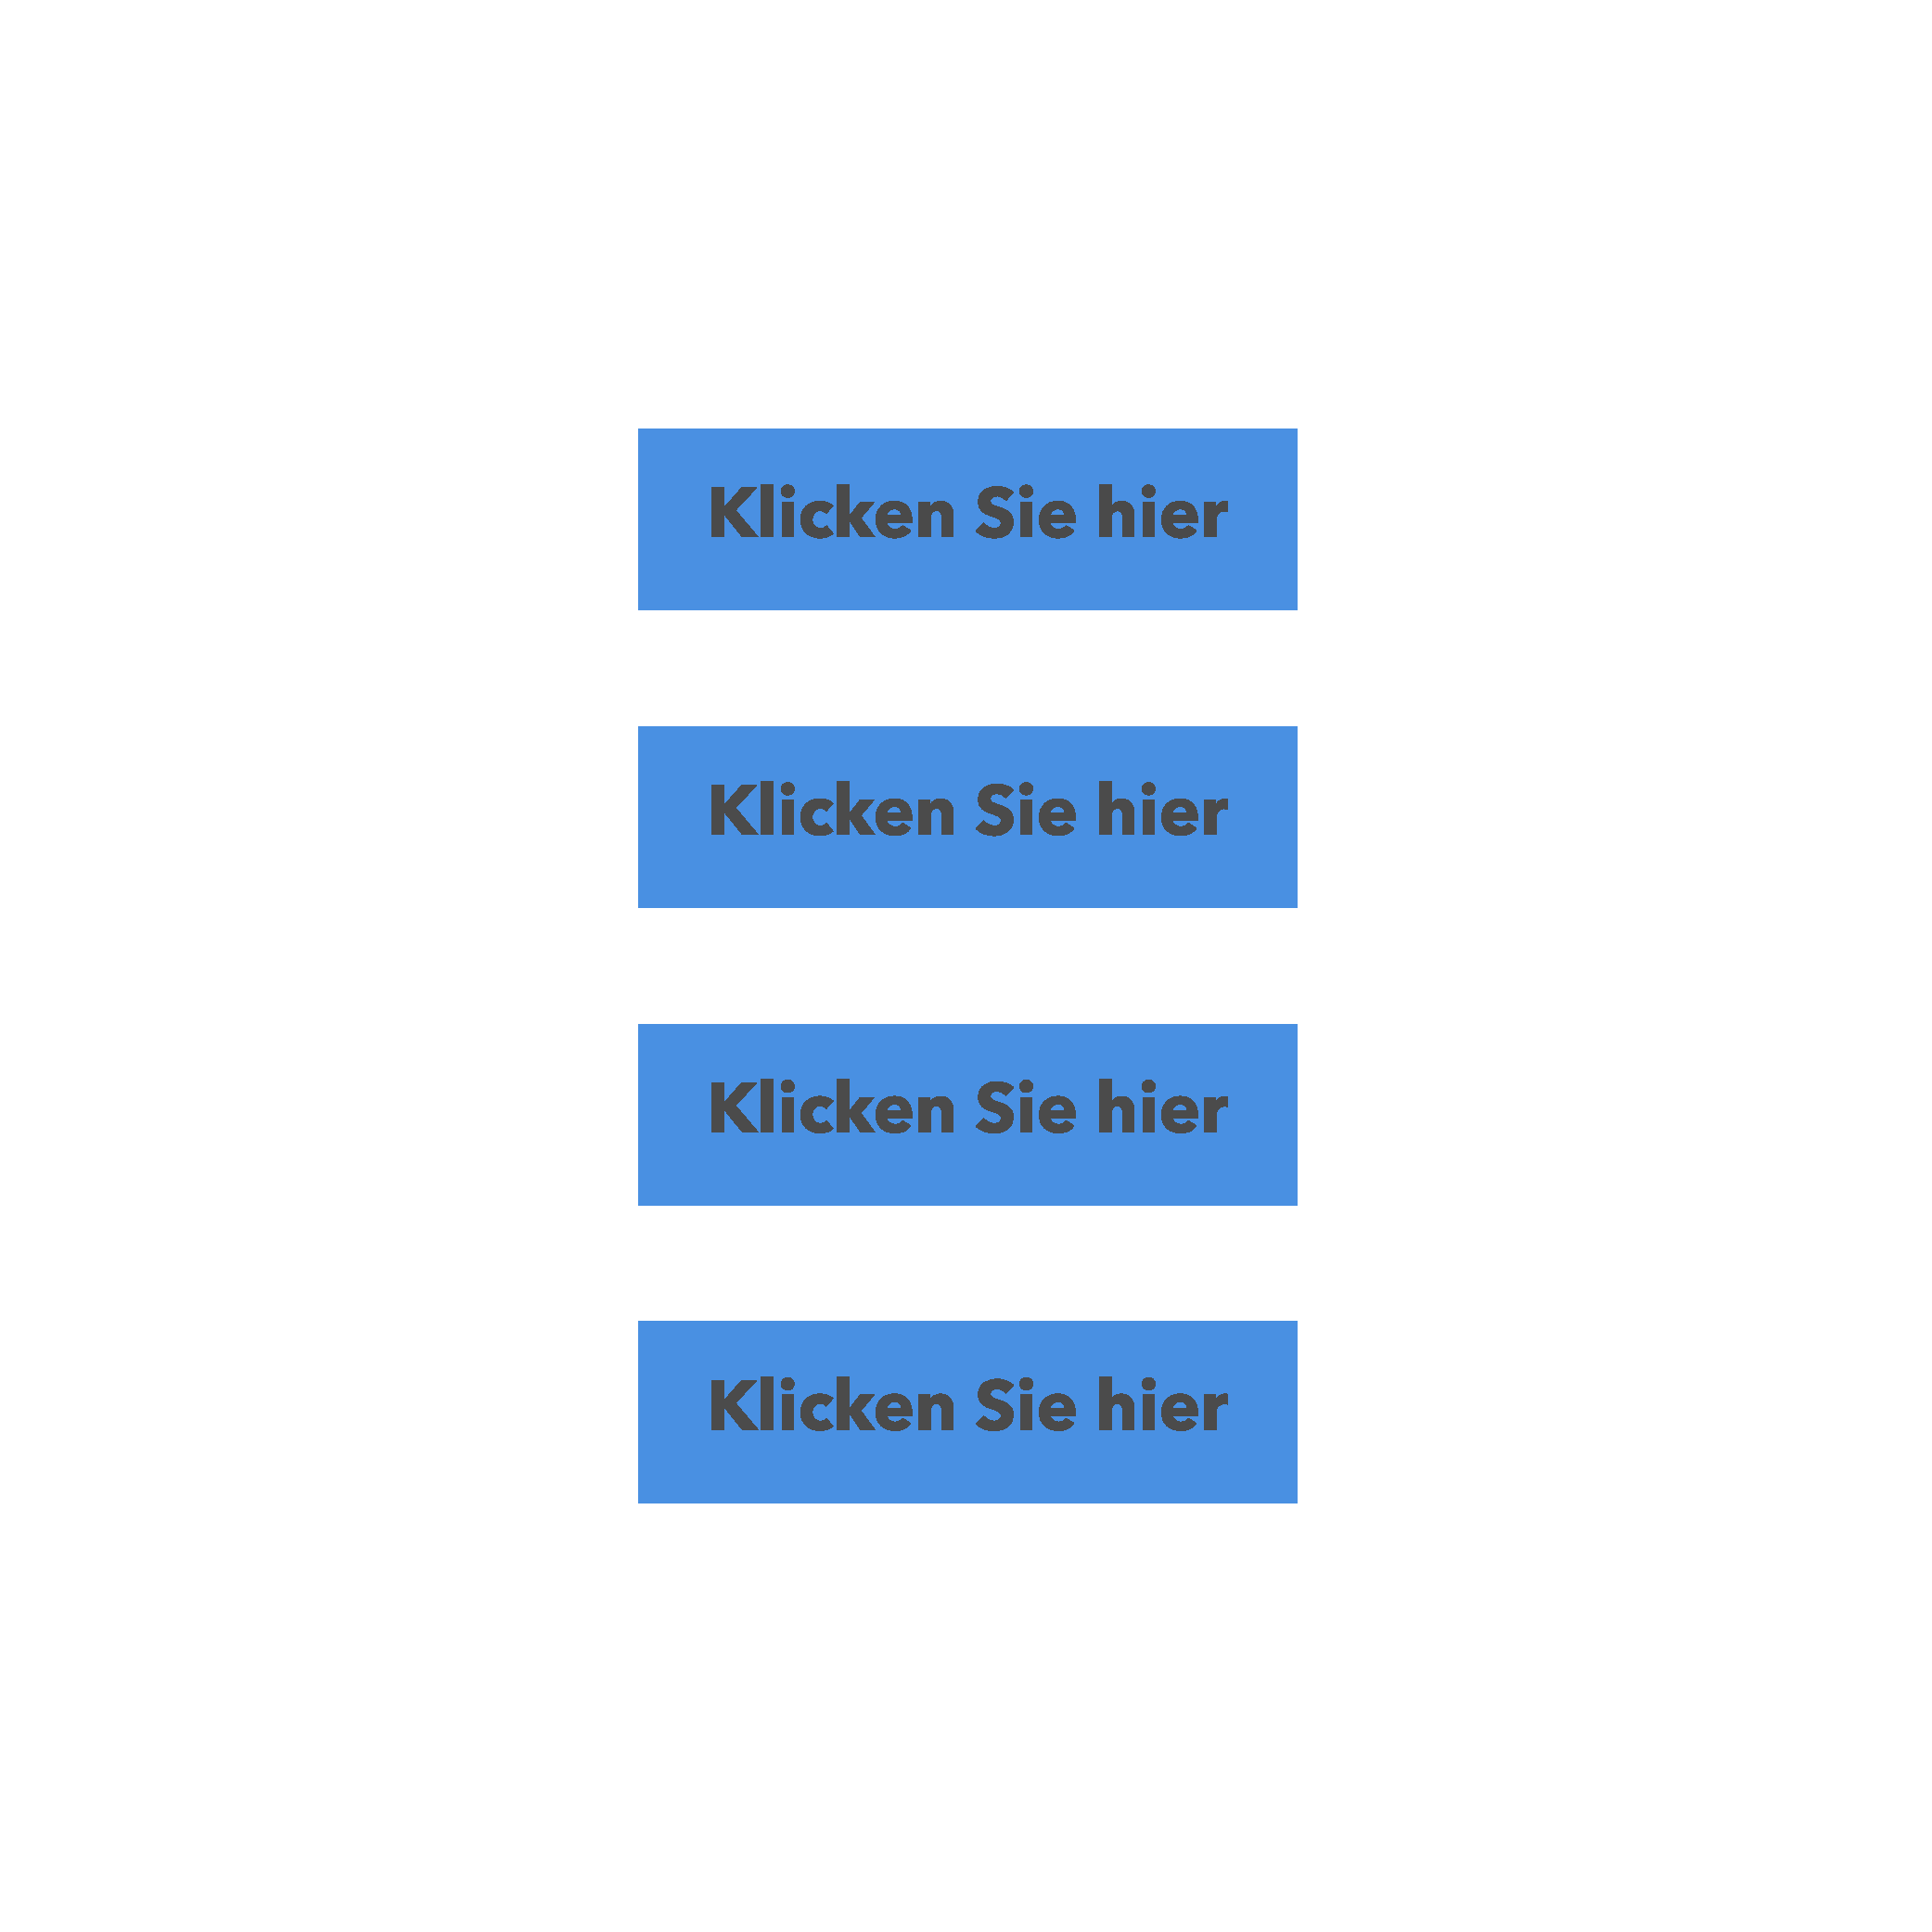
\includegraphics[width=0.60\textwidth]{images/sample_schatten.pdf}
}
\caption[Unterschiedliche Schatten an Buttons]{Unterschiedliche Schatten an Buttons\\ Eigene Darstellung}
\label{sample_schatten}
\end{figure}

\subsection{Vertraute Größe}
\marginnote{DD}
Die vertraute Größe - oder auch relative Größe - erlaubte es, sofern die echte Größe des betrachteten Objekts bekannt ist, die Entfernung zum Objekt zu schätzen. Dies geschieht anhand einer Unterscheidung zwischen der realen Größe und der relativen Größe des Objektes. So können auch gleiche Objekte mit unterschiedlichen relativen Größen als verschieden Weit entfernt erkannt werden.\footcite[Vgl.][S.43]{Ass16}

\vspace{1em}
\begin{minipage}{\linewidth}
	\centering
	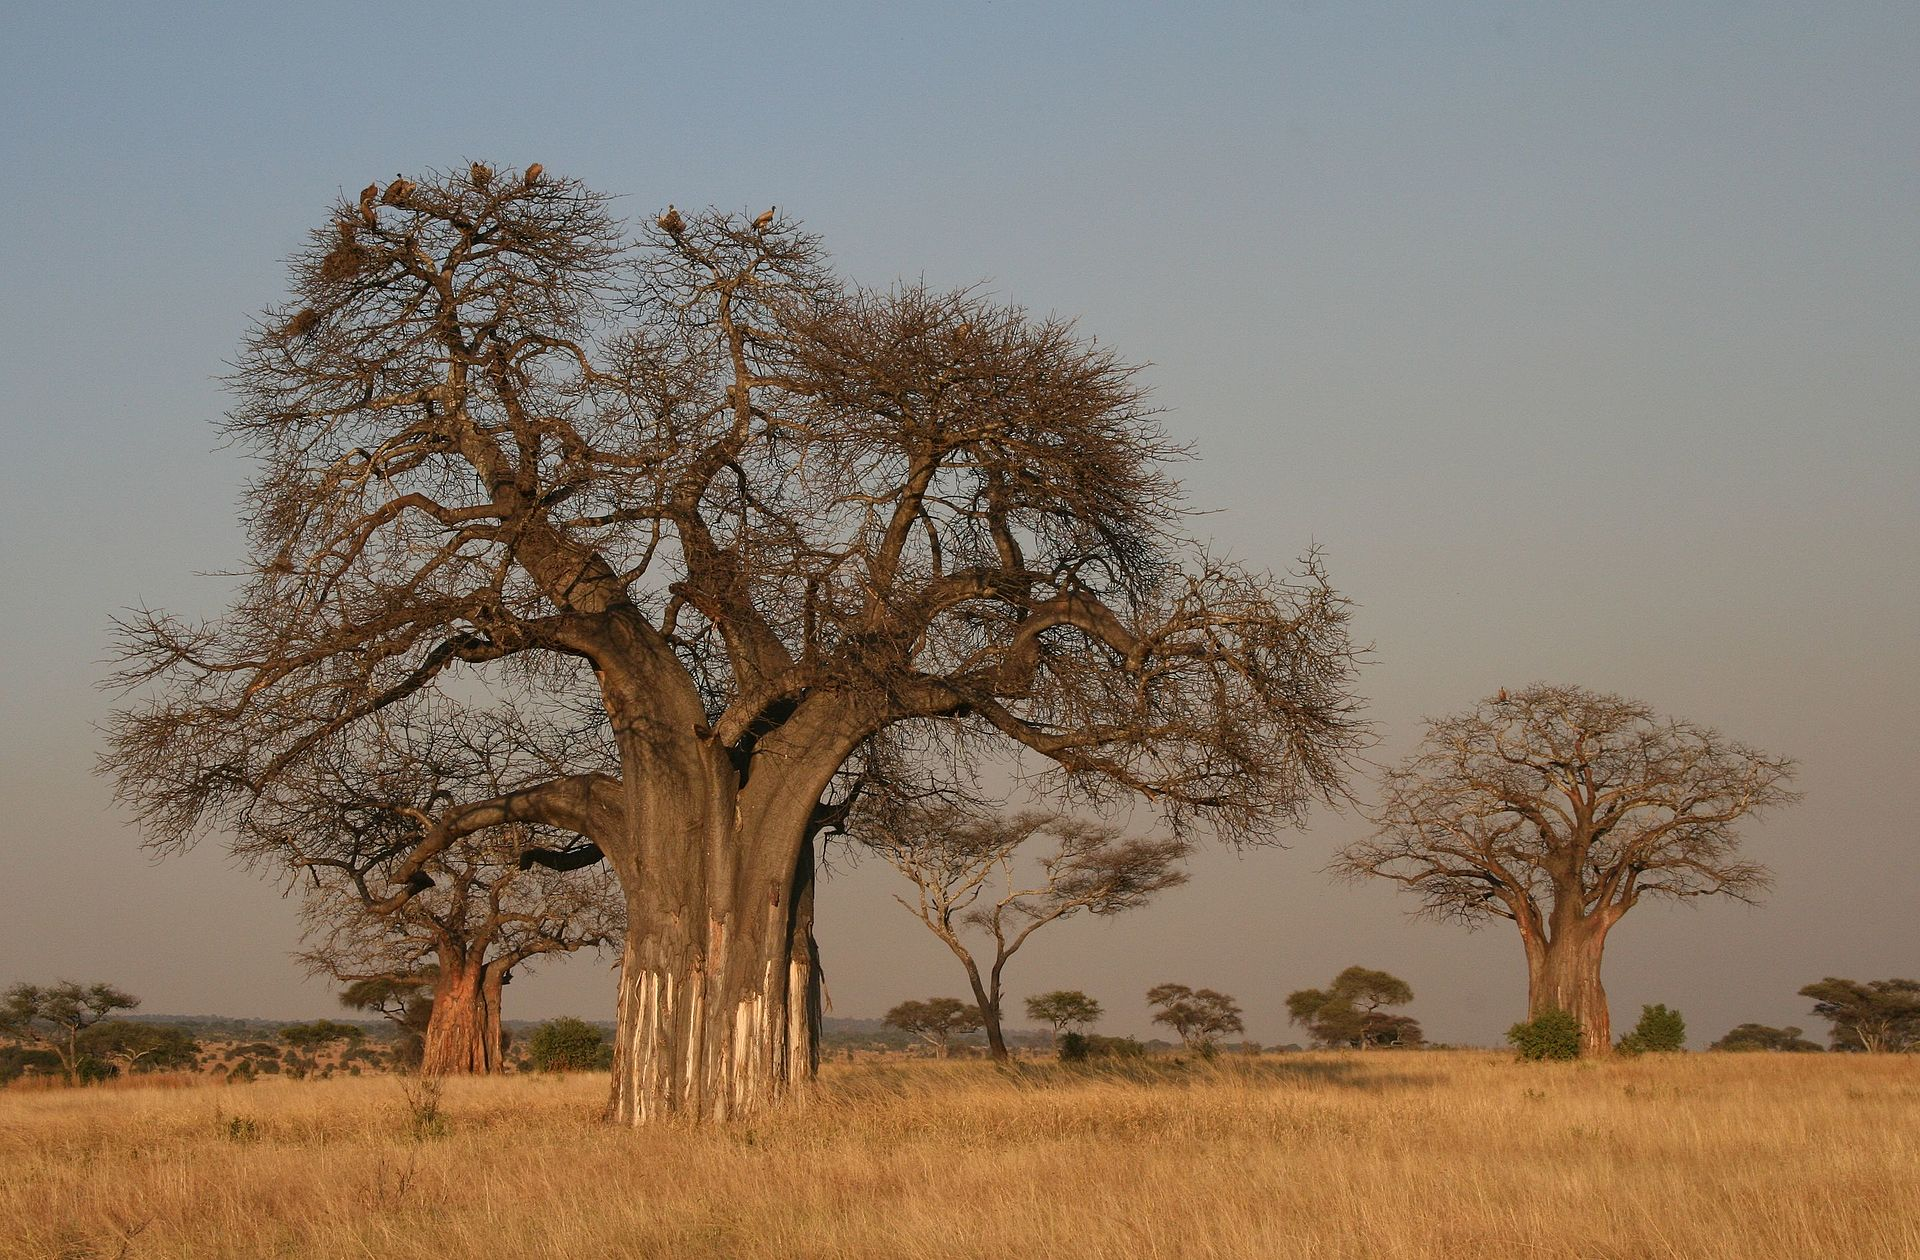
\includegraphics[width=0.7\linewidth]{images/baeume.jpg}
	\captionof{figure}[baeume]{Baumlandschaft (\cite{yokyXX})}
	\label{fig:baeume}
\end{minipage}
\vspace{1em}

Die Abbildung \ref{fig:baeume} verdeutlicht das Kriterium der vertrauten Größe. Es zeigt eine Landschaft mit Bäumen, die unterschiedlich Groß sind. Die kleineren Bäume geraten aufgrund des Kriteriums der vertrauten Größe automatisch in den Hintergrund und die größeren Bäume in den Vordergrund. Demnach erscheinen die größeren Bäume näher zum Betrachter.\\
\\
Ein interessanter Fakt zu diesem Kriterium ist, dass die vertraute Größe auf langjähriger Erfahrung beruht. Aus diesem Grund schätzen besonders Kinder die Größe von Objekten in ihrer Umgebungen sehr abweichend von der tatsächlichen Relation ein. \footcite[Vgl.]{Helm1867}
\begin{figure}[!ht]
\centering
\fbox{
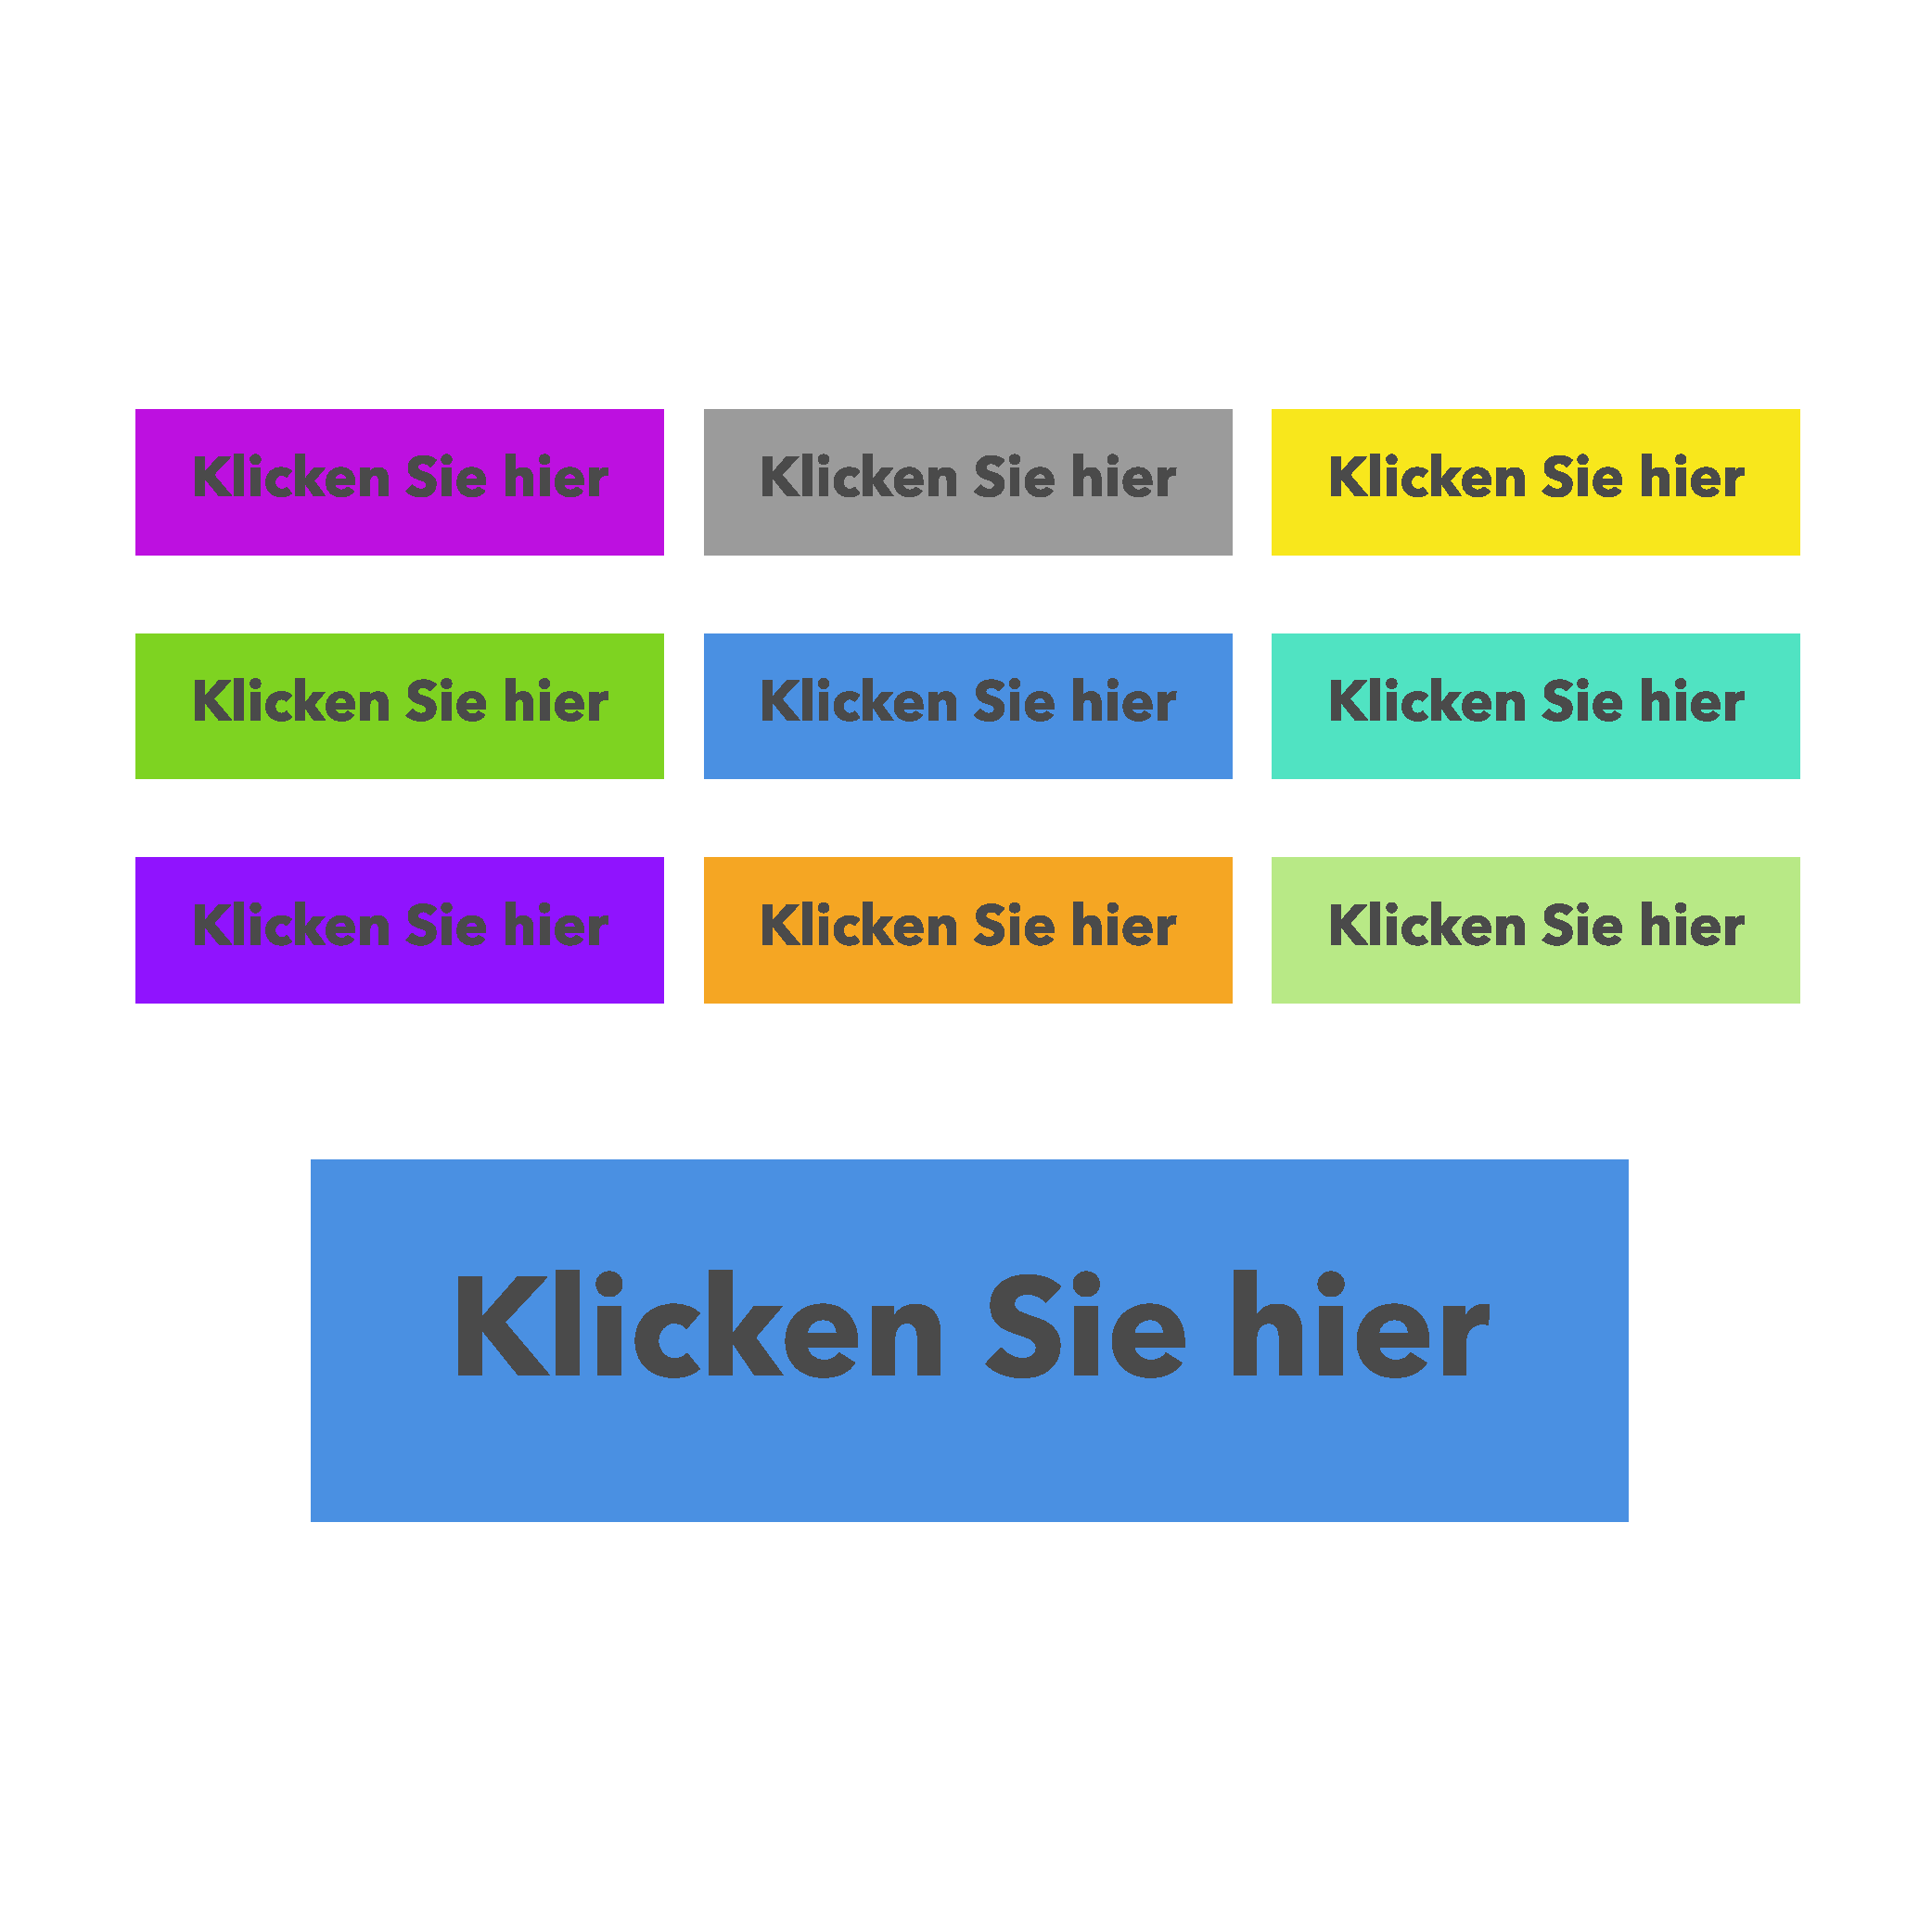
\includegraphics[width=0.60\textwidth]{images/sample_vertraute_groesse.pdf}
}
\caption[Vertraute Größe von Buttons	]{Vertraute Größe von Buttons\\ Eigene Darstellung}
\label{sample_vertraute_groesse}
\end{figure}

\subsection{Relative Helligkeit und perspektivische Unschärfe}
...
\begin{figure}[!ht]
\centering
\fbox{
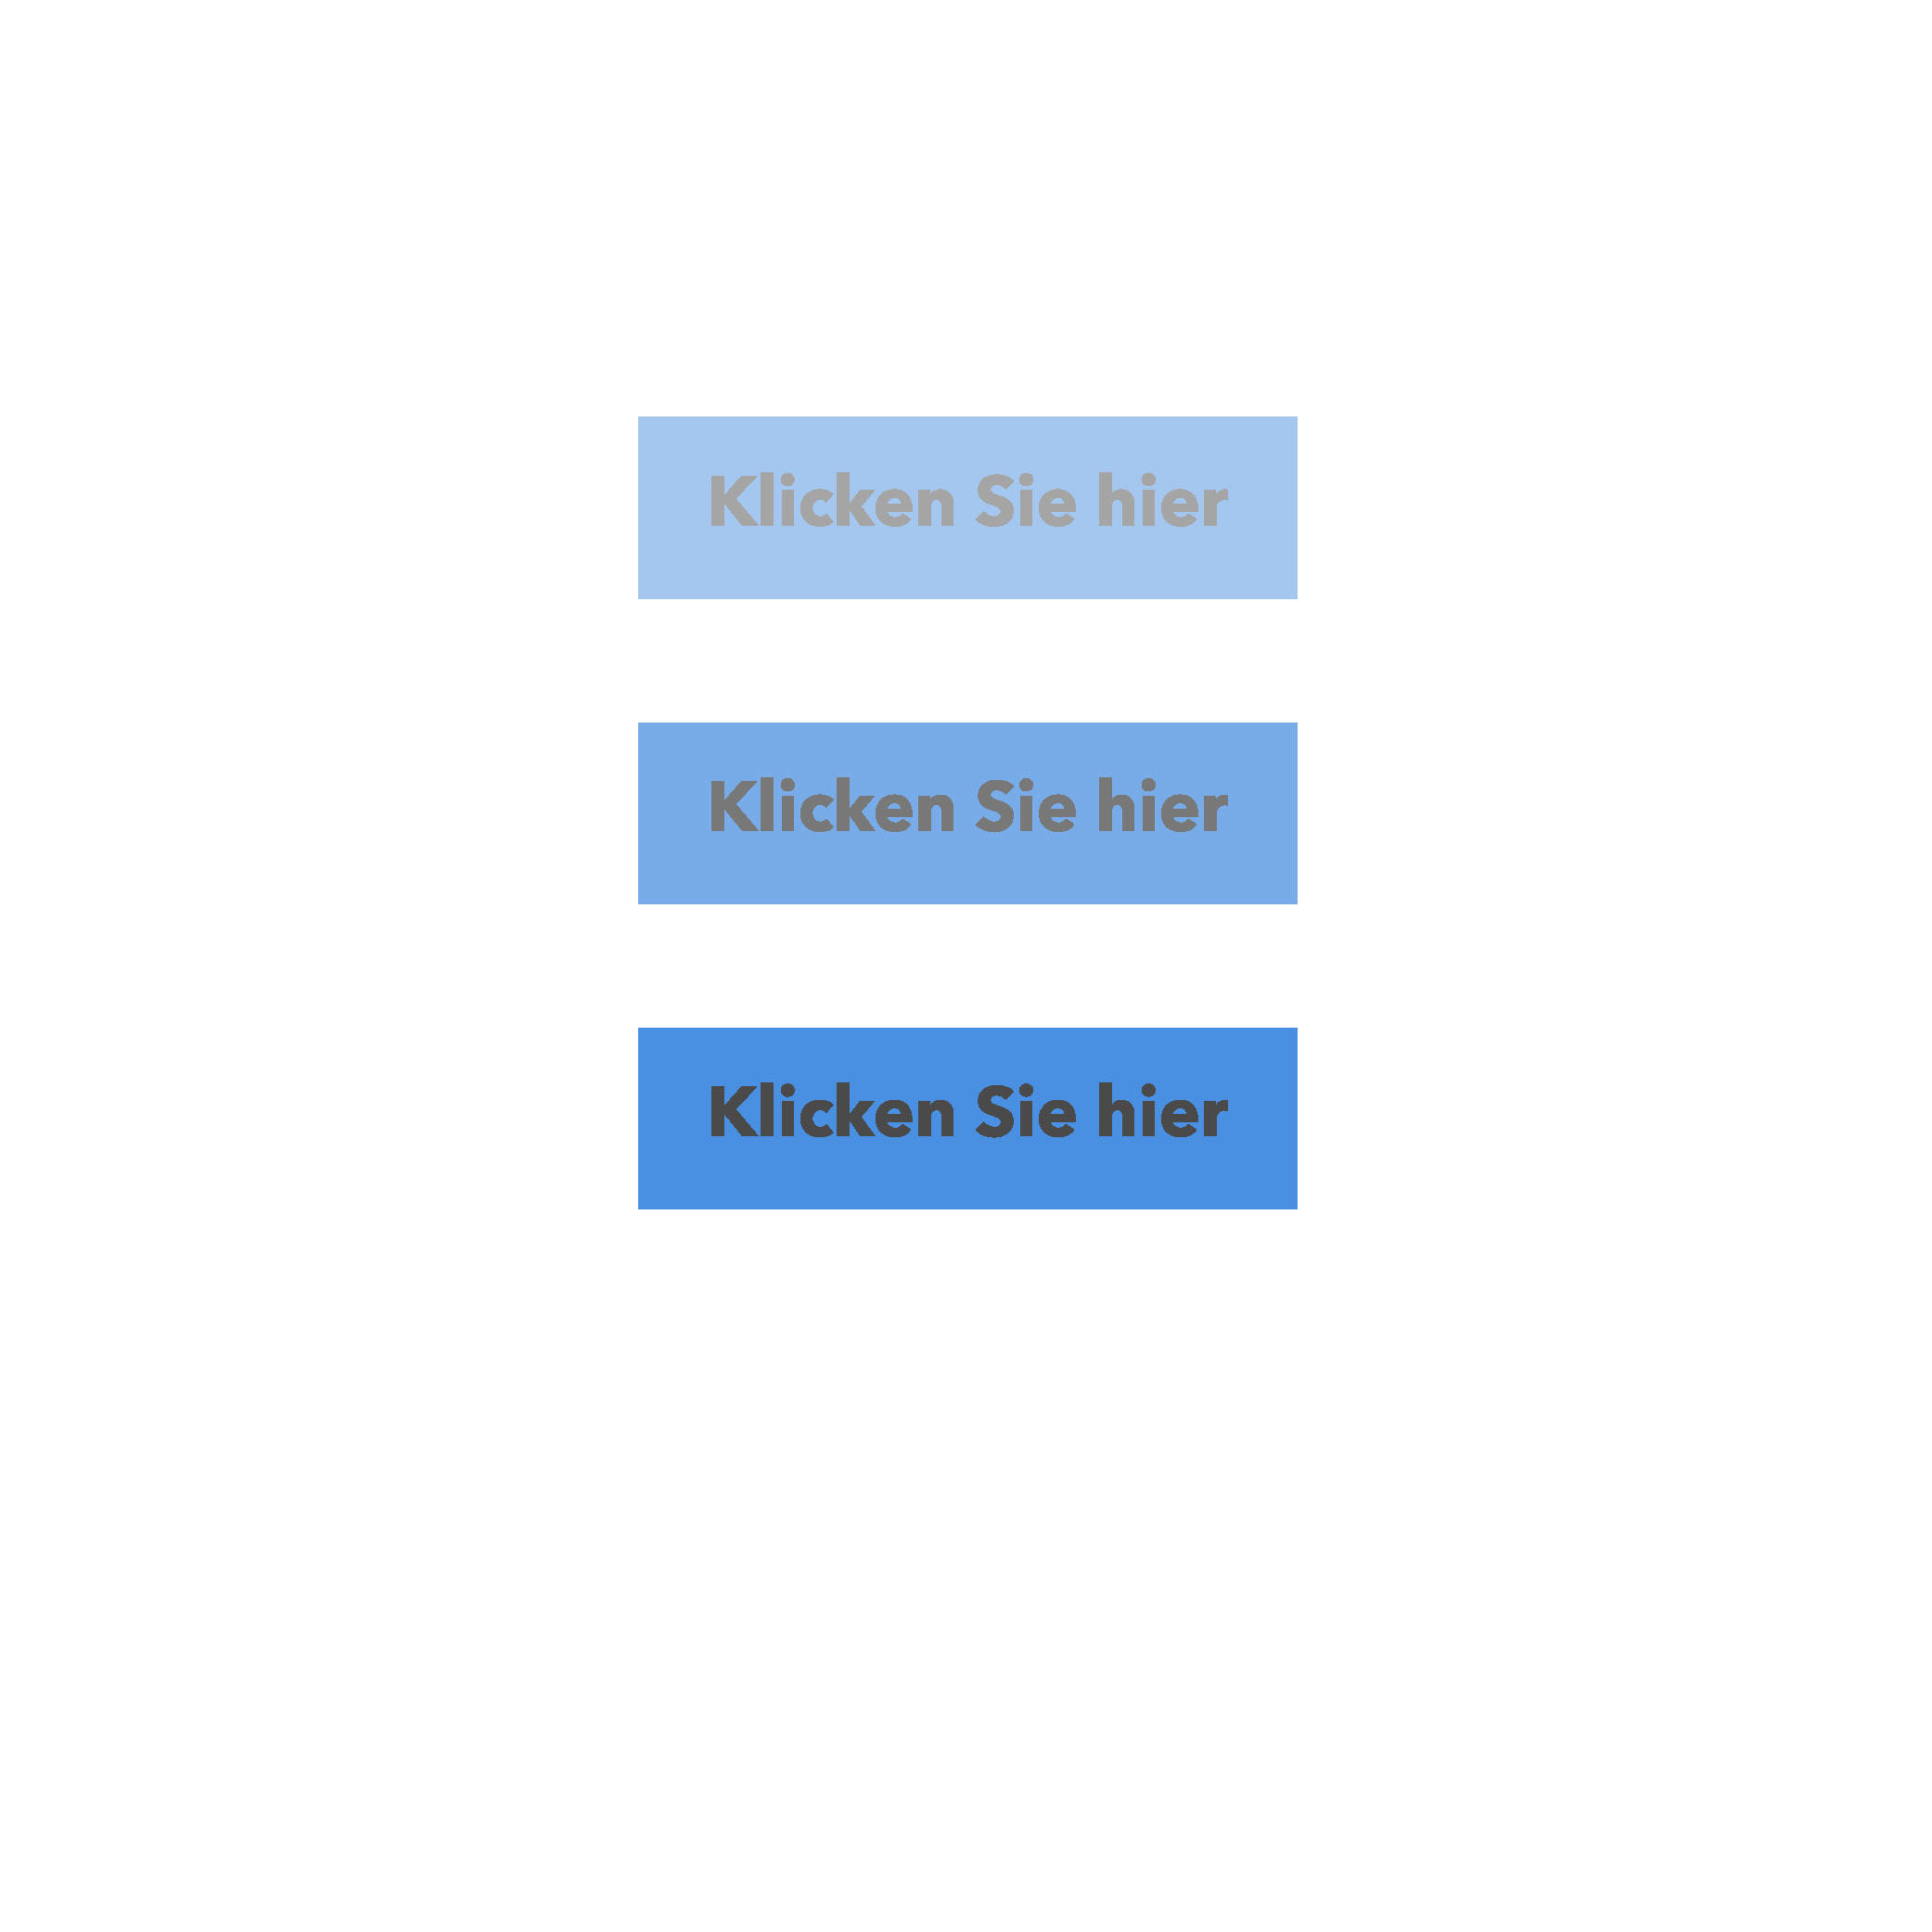
\includegraphics[width=0.60\textwidth]{images/sample_relative_helligkeit.pdf}
}
\caption[Relative Helligkeit von Buttons]{Relative Helligkeit von Buttons\\ Eigene Darstellung}
\label{sample_relative_helligkeit}
\end{figure}


\subsection{Texturdichte-Gradient}
...
\begin{figure}[!ht]
\centering
\fbox{
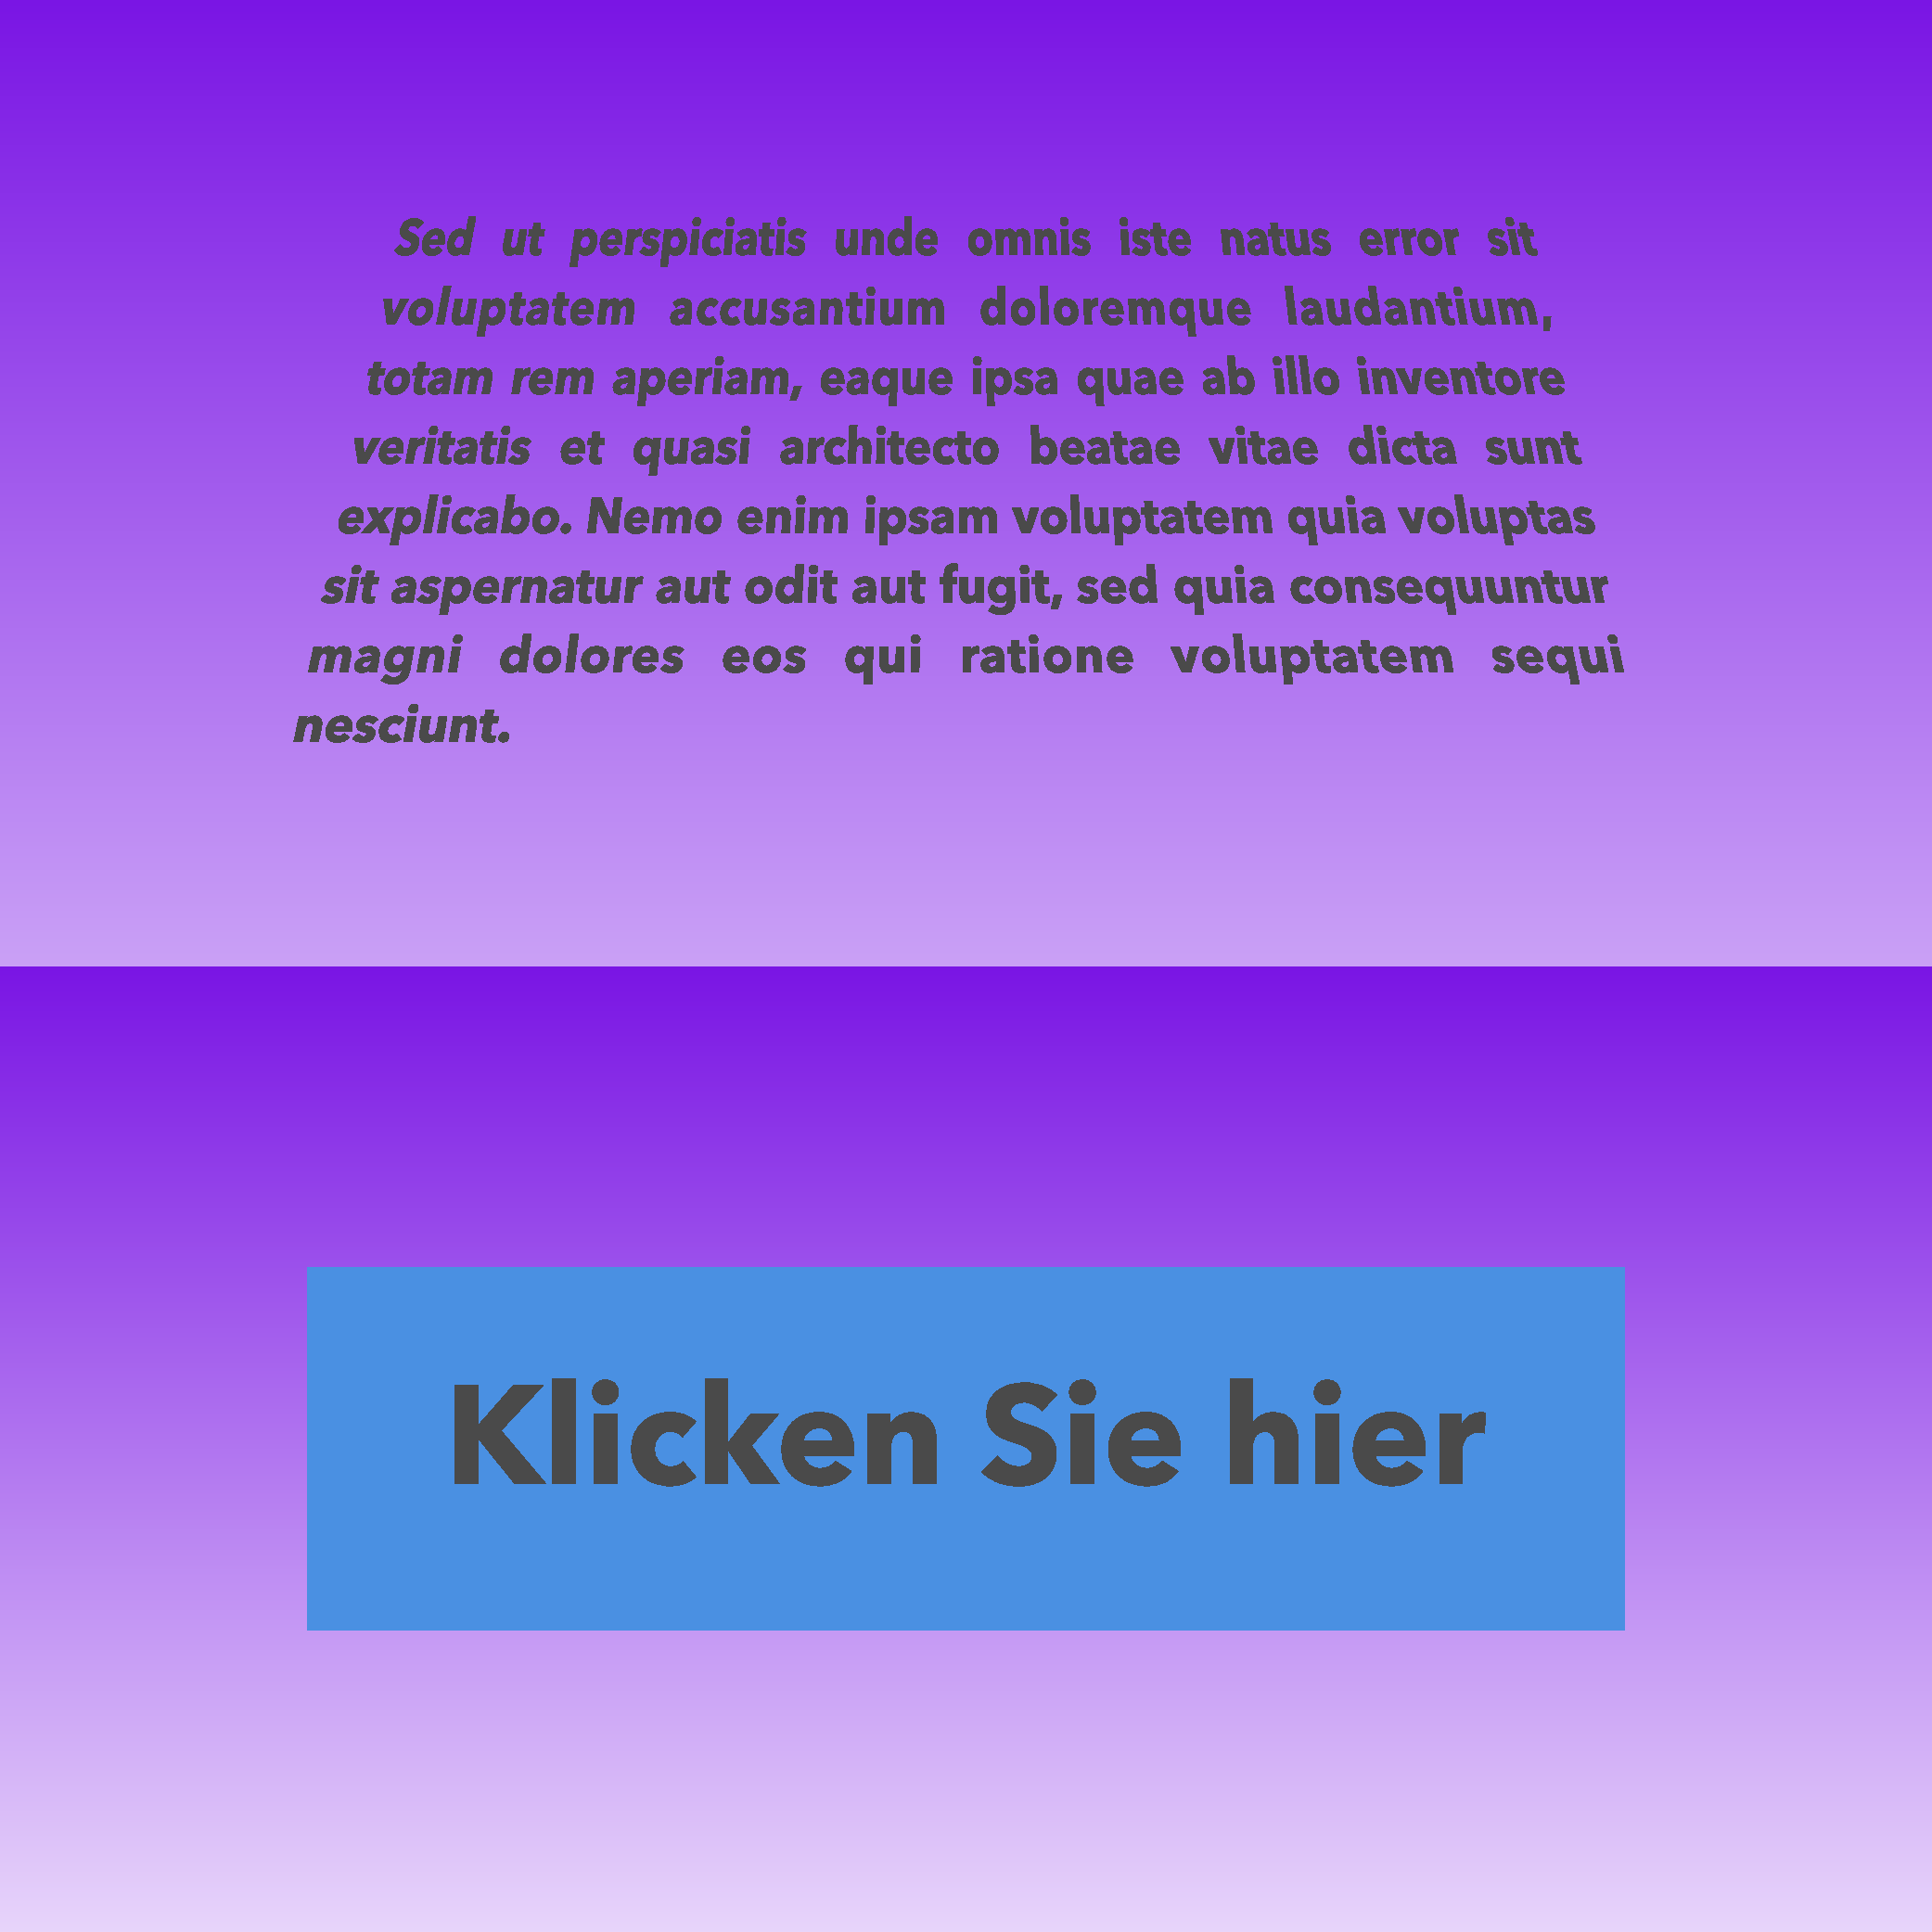
\includegraphics[width=0.60\textwidth]{images/sample_texturgradient.pdf}
}
\caption[Texturgradient im Hintergrund]{Texturgradient im Hintergrund\\ Eigene Darstellung}
\label{sample_texturgradient}
\end{figure}


\subsection{Lineare Perspektive}
...

\begin{figure}[!ht]
\centering
\fbox{
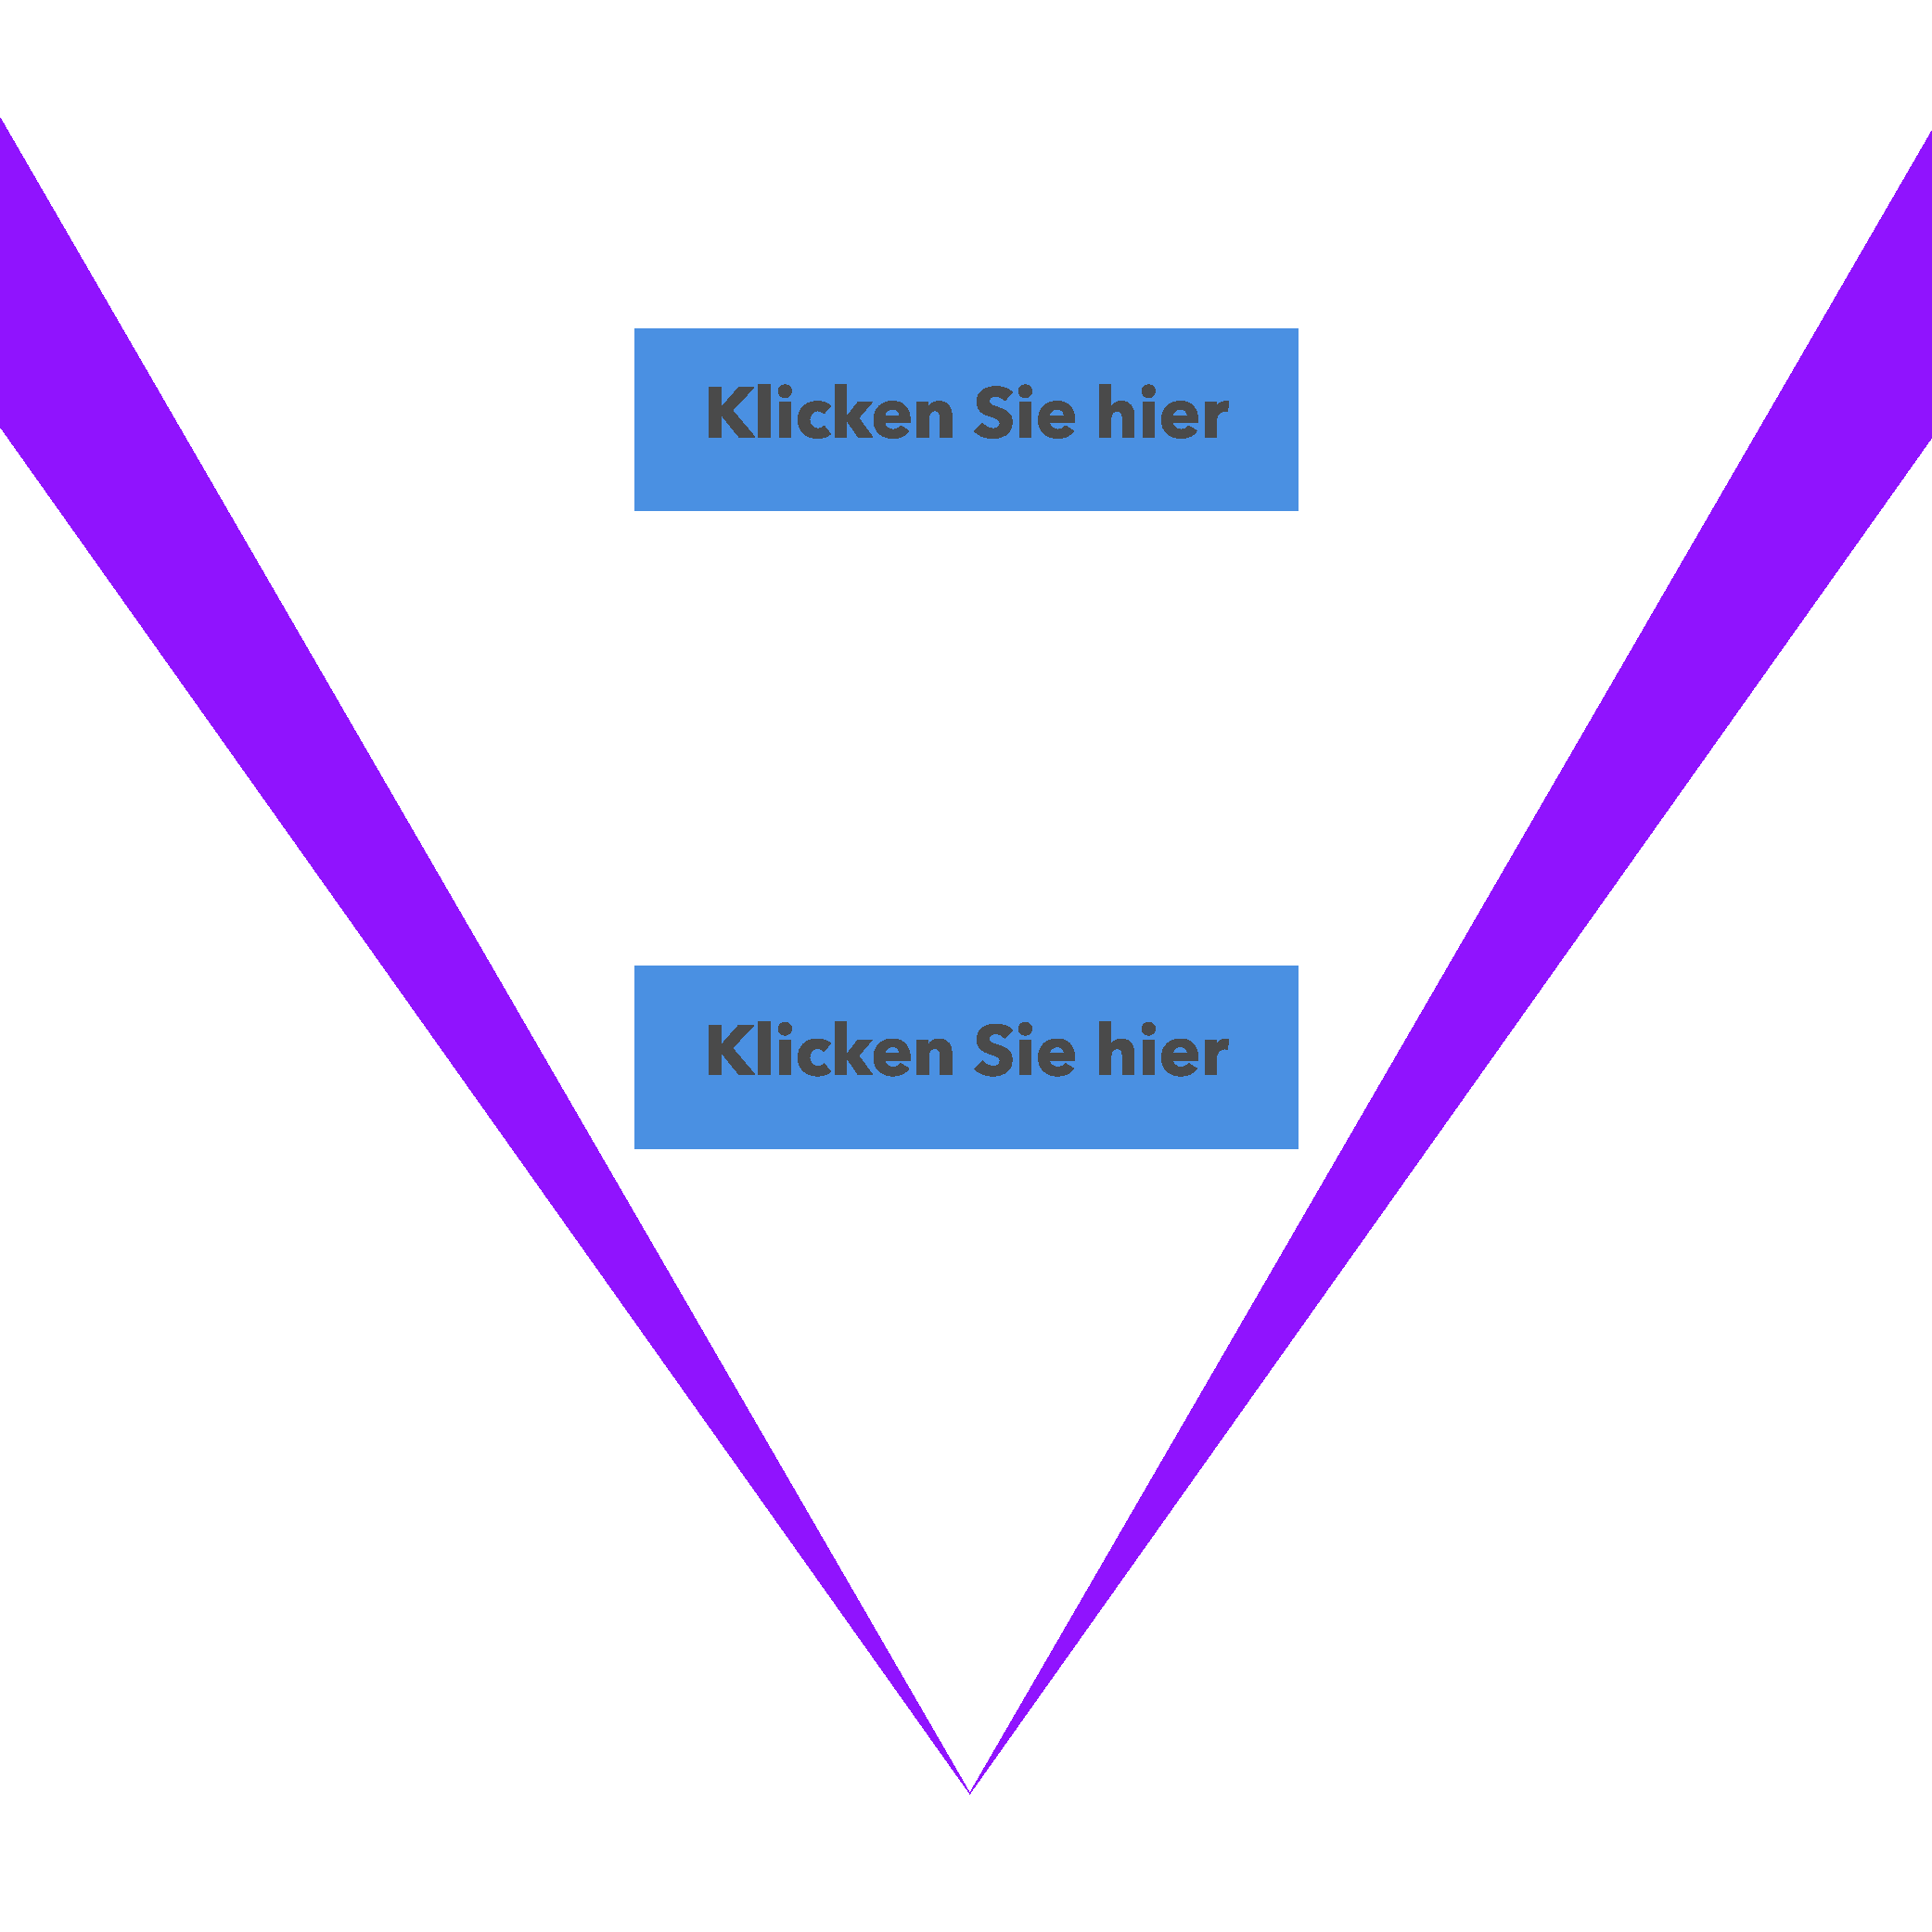
\includegraphics[width=0.60\textwidth]{images/sample_lineare_perspektive.pdf}
}
\caption[Lineare Perspektive]{Lineare Perspektive\\ Eigene Darstellung}
\label{sample_lineare_perspektive}
\end{figure}

\subsection{Relative Höhe / Lage zum Horizont}
...

\begin{figure}[!ht]
\centering
\fbox{
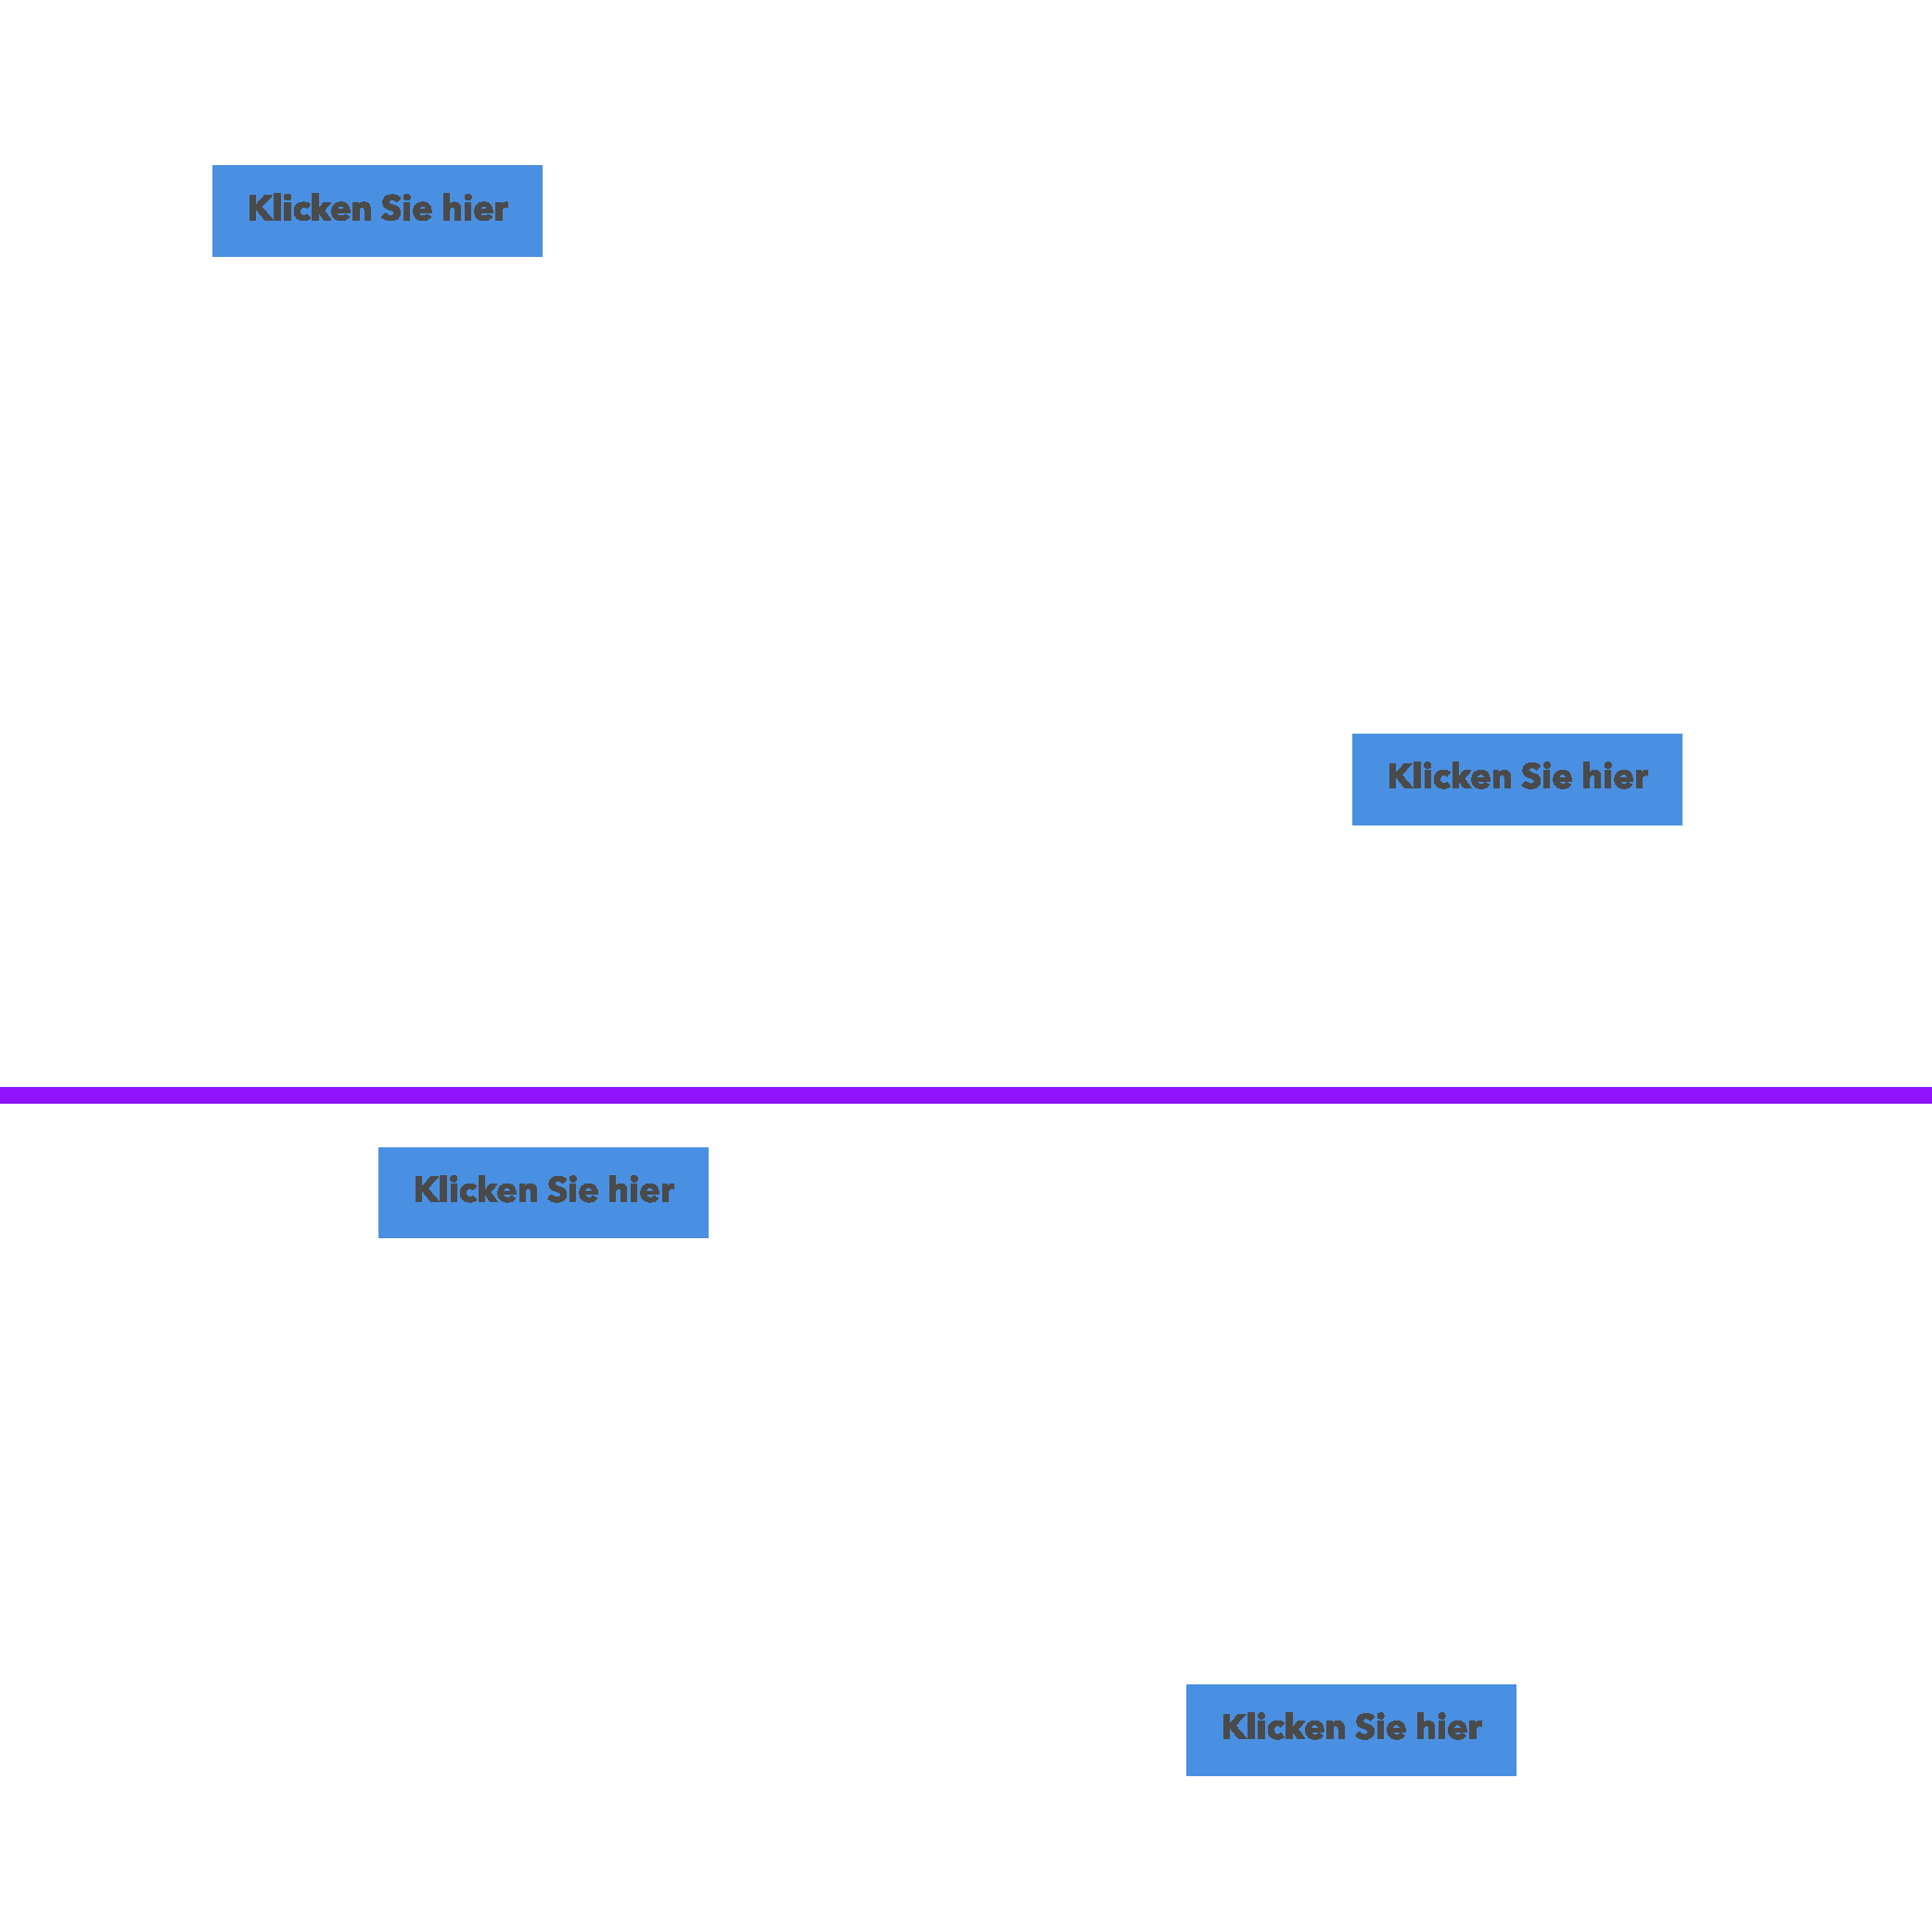
\includegraphics[width=0.60\textwidth]{images/sample_lage_zum_horizont.pdf}
}
\caption[Lage zum Horizont über künstlichen Horizont]{Lage zum Horizont über künstlichen Horizont\\ Eigene Darstellung}
\label{sample_lage_zum_horizont}
\end{figure}

\subsection{Abgrenzung zu binokularen Tiefenkriterien}
...

\subsection{Bewegungsparallaxe}
...

\section{Konzeption}
...

\section{Umsetzung}
...

\section{Zusammenfassung}
...